
% Differential treatment of Interests received from different interfaces can be achieved in a more elegant way, without reverting to probabilistic methods.

The previous algorithm---the satisfaction-based Interest acceptance---divides the available forwarding tokens among all interfaces in proportion to their Interest satisfaction ratios.
% Given the drawbacks of this algorithm, the same effect can be achieved without relying on probabilistic models. 
An alternate algorithm for proportional token distribution without overreaction is to enable and enforce explicit Interest limit for each incoming interface, where the value of the limit depends directly on the interface's Interest satisfaction ratio.
Routers need to announce these limits to their downstream neighbors, ensuring that any Interest forwarded from the downstream router is allowed to get through, resulting in genuine Interest satisfaction statistics.

The formal definition of the satisfaction-based pushback algorithm is presented in Pseudocode~\ref{alg:dynamic limits}, while Fig.~\ref{fig:dynamic limits example} illustrates how the algorithm will work in our example in Fig.~\ref{fig:flooding example}.
Assuming an initial token bucket limit $L=10$ and the current satisfaction ratio for router A is 50\% for \texttt{eth1} and 0\% for \texttt{eth0}, and for router B the ratio is 30\% for \texttt{eth0}, each node will set and announce the following  incoming interface limit $L'$: 
\begin{enumerate}
\item router B will set and announce the incoming interface limit $L'=3$;
\item router A, after receiving announcement from B will readjust its incoming interface limits to $L'_{eth1} = 1.5$ and $L'_{eth0} = 0$; and
\item both legitimate users and adversaries may either obey or ignore the announced limit, which will be in any case enforced by router A.
\end{enumerate}


\begin{figure}[htbp]
  \centering
  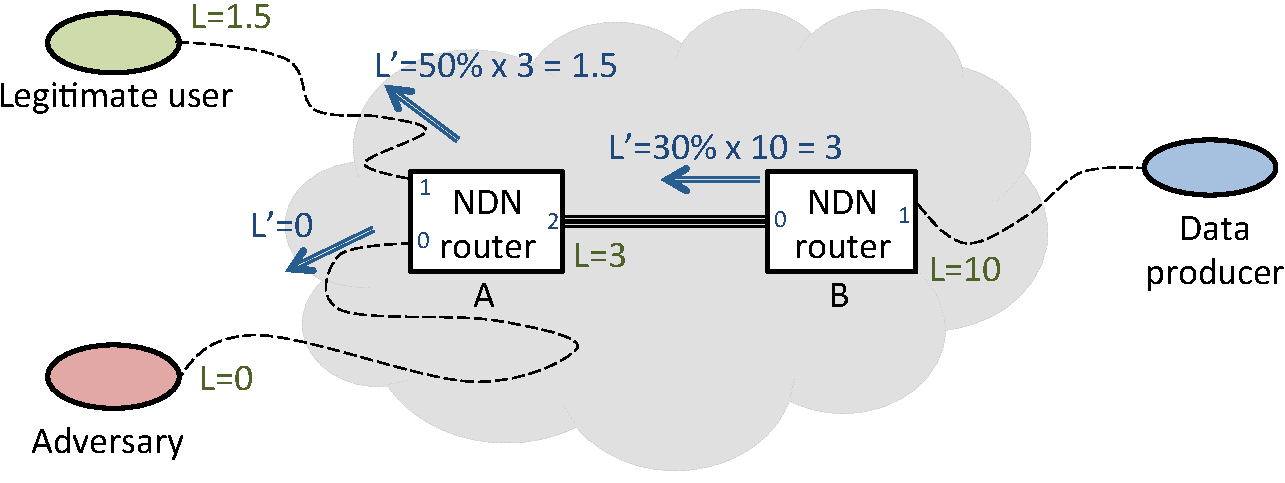
\includegraphics[scale=0.3]{dynamic-limits}
  \caption{Satisfaction-based pushback example
%: routers explicitly tell neighbors how many Interest packets they can deliver to the Data producer%
}
  \label{fig:dynamic limits example}
\end{figure}


\floatname{algorithm}{Pseudocode}

%%%%%%%%%%%%%%%%%%%%%%%%%%%%%%
%%%%%%%%%%%%%%%%%%%%%%%%%%%%%%
%%%%%%%%%%%%%%%%%%%%%%%%%%%%%%
{ 
\begin{algorithm}[h]
\footnotesize
\caption{\small Satisfaction-based pushback}
\label{alg:dynamic limits}
\begin{algorithmic}[1]
% \State{}\Comment{Same initialization, InData and Timeout functions as in Pseudocode~\ref{alg:queuing}}
\State{} \Comment{Same init, InData and Timeout functions as in Pseudocode~\ref{alg:queuing}}
\vspace{0.1cm}
\State{$\forall f \in \mathrm{interfaces} : L'_{f} \leftarrow L_{f}$} \Comment{Per-incoming interface Interest limit} 

\vspace{0.1cm}

\State{} \Comment{\textit{Announcement from the neighbor}}
\Function{InLimits}{InInterface $in$, Limit $L'$}
    \State $L_{in} \leftarrow L'$
\EndFunction

\vspace{0.1cm}

\Function{AnnounceLimits}{} \Comment{\textit{E.g., every second}}
\For{\textbf{each} outgoing interface $out$}

   \For{\textbf{each} incoming interface $in$}
        \State $L'_{in}= {L_{out}} \times (1 - U_{in}/F_{in})$
        \State AnnounceLimit($in$, $L'_{in}$)
   \EndFor

\EndFor
\EndFunction

\end{algorithmic}
\end{algorithm}


The zero limit for the adversary's link implies that  router A is temporarily not willing to accept any Interests from this interface until the statistics decay to the appropriate level (recall Fig.~\ref{fig:ratio example}).
At the next iteration of the satisfaction-based pushback algorithm, the legitimate user will be able to gradually improve the statistics on both routers A and B as all Interests from the user will get through and will return Data, eventually resulting in a full allowance ($L'=L=10$) in the links between the routers A and B, and the user and router A.

We note that while in the description of the satisfaction-based pushback algorithm we explicitly used ``outgoing'' and ``incoming'' interfaces,  all interfaces can be both incoming and outgoing.
Thus, it may not be entirely clear which outgoing limit $L_{out}$ (line 10 in the algorithm) should be used to calculate the incoming limit $L_{in}$.
To overcome this problem, in our actual implementation we enforced separate incoming/outgoing interface limits for each individual FIB entry.
That is, for each FIB entry we set a separate Interest limit for each incoming interface (${L'}_{in}^{fib}$) based on a sum of FIB entry limits for each outgoing interface $L=\sum{L_{out}^{fib}}$.


Both satisfaction-based Interest acceptance and satisfaction-based pushback algorithms are forms of a well-known push-back mechanism~\cite{Pushback}, but with several core differences. 
First, we are suppressing (pushing back) unwanted requests for Data, not actual Data itself.
Second, differentiating between good and bad Interests is based on the traffic symmetry principle of NDN.
% Alex: I'm not entirely sure about this point... 
Finally, both intelligent attack mitigation algorithms can be deployed at all times without degrading network performance even when there are no active attackers. 


%%% Local Variables: 
%%% mode: latex
%%% TeX-master: "../paper"
%%% End: 
